\documentclass[twoside,10pt]{article}
\usepackage{amsmath,amsfonts,amsthm,fullpage}
\usepackage{mymath}
\usepackage{algorithm}
\usepackage{algorithmic}
\usepackage{graphicx}


\begin{document}

\title{Special Problem Mathematical Equations}
\author{}
\date{}
\maketitle


Spatial Optimization is one of the most important problem in computational sustainability today. For the purpose of understanding ,we can consider that if we are given a raster matrix (M*N), spatial optimization can be described as allocation of land types (Commercial, Residential, Green,Industrial, Recreational) to each of the cells /land mass under given constraints (money, contiguity, future expansion etc.).  Spatial Optimization is challenging because it involves lots of dependencies, variables, objectives and input parameters. And as these features increase the problems becomes more complex and it grows exponentially. Solving such a massive problem manually is out of question. We need computational tools to better understand all the aspects of such a gigantic problem.
Comprehensive sustainability in urban planning can be termed as a long-term balance between economic development, environmental protection, efficient resource use, and social equity


Spatial Optimization can also be looked as a demand-constraint problem, where objective is to allocate land type of given land masses keeping in mind the various constraints. The abstract concept of constraints on which  desired constraints and objectives are build are :-
Continuity
Compactness
Compatibility

\graphicspath{ {images/} }
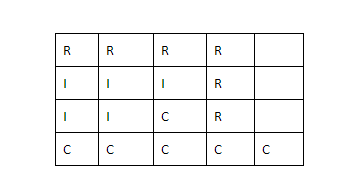
\includegraphics{raster}

\subsubsection*{Continuity} - Continuity can be defined as as the degree to which a specific use has been allocated to land in an unbroken fashion. It basically refers to the connected component of the same type. Here, in the figure we can see that C has very high contiguity.

\subsubsection*{Compactness} - We define compactness as an allocation of a given land use to sites that are in direct proximity of each other, resulting in circular patches. In the figure above, we can see that land type I has maximum compactness.

\subsubsection*{Compatibility} - Compatibility  as the word suggests refers to how compatible a given land use type is with his neighbour(other land type) . We would prefer to have green areas close to residential as compared to having industry close to residential, thus compatibility index of the former will be higher.

In a land usage optimization problem, finite amount of resources (commercial, industrial, residential area etc.) are allocated effectively to a specific land mass under given constraints (money, contiguity, future expansion etc.). In fact it has been depicted that inefficient resource use leads to high traffic congestion and other sustainability issues (Newman et al.). Therefore, it is important to carefully design land use allocation models. Since, land use allocation is a resource allocation problem for a given space, therefore many times it is considered as a spatial optimization problem. This problem was first addressed by Schlager et al. as a Linear Programming model in 1965 and it was mostly constrained to single objective optimization. Since this problem is much more complex and involves a lot more objectives, therefore multi-objective approach was adopted by other researchers (mentioned in following section).  Many researchers however constrained themselves by still continuing with Linear Programming approach and by assigning different weights to different objectives and performing linear combinations to attain the solution.It is a major issue for planners to numerically quantify the relative weights of each of the defined objective. Moreover, non-convex optimal solutions cannot be obtained by minimizing linear combinations of objectives.


Due to the multifaceted nature of land-use allocation, spatial optimization modelling should aim at finding a set of high-performing alternatives instead of just one solution (Bankes 1993, Church 1999, Harris 2001) and allow the stakeholders to choose from a number of scenarios that are both good and different from each other, since not every planning objective of interest may be introduced into the
model in the form of mathematical formulation (Chang et al. 1983, Brill et al. 1990). The decision-makers should be provided with alternatives that allow for consideration of other—less defined—planning goals, or recognition of overlooked issues and innovative solutions (Chang et al. 1983). Consequently, the generated alternatives should be treated not as ultimate solutions but as propositions for further analysis by stakeholders.

\subsubsection*{Conventions}
Let us first define the conventions we will use for variables . \\ 
\begin{itemize}
\item Landuse : Landuse specifies the type of land allocation to that particular area. They can take values from 0 to N, where N is the number of landuse types. We will always refer to 0 as the undeveloped land type and others would be enumerated depending upon the number of land types available. To refer to particular area we will use the notation $X_{ik}$, where land/pixel i is assigned a landuse type k.
\item Attractiveness : We define $a_j$  as the measure of attractiveness of an undeveloped location for development. 
$ a \in (0,1)$
\item Area : $A_j$ is the area of the parcel j.
\item $Y_i$ is the initial land use type of parcel $i \in V$
\item V : Refers to all the parcels /cells

\item U : Refers to set of parcels that are undeveloped \\
 
$ Y_{i} = 0$ , where  $Y_{i}$ refers to the land use type. 
\item $N_j$ : Neighbours of parcel $j \in V$    
\item Compatibility : $\partial_{kk'}$ refers to compatibility of landuse type k with k', where k,k' $\in {0,..N}$
\item : Closest Neighbour -  $dist_j$ refers to distance from j to closest developed neighbour cell.
\item $\vartheta_{kk'} $ - Refers to the conversion cost from  type k to k'
\item $s_j$ : Number of initially developed neighbours of j , $$ s_j = \sum_{i \in N_j: Y_i \neq 0} 1$$
\item $rd_j$ : road distance to the closest road from cell  j
\item roadDist(dis,k) : It is the penalty for distance from road for type k


\item
\subsubsection*{Minimize Undeveloped Land}

We define $ a_{j},$ as the attractiveness of an undeveloped location for development. Higher value indicates higher attractiveness towards development.  Thus, we can have low value for undeveloped open places. and minimize the following

 $$
 min\sum_{j \in U} (1-a_j) \sum_{k=1}^N X_{jk}
 $$
Consider values $a_j$  for all cells that encode attractiveness for development for undeveloped cells. Idea is to set $a_j$ very low for cells in open space. Add objective to minimise summation of (1-$a_j$) for all undeveloped cells that are developed. 

\item 
\subsubsection*{ Compatibility(special version of contiguity)}
We would like to maximize compatibility of a cell wrt its neighbours.
 $$
max \sum_{j \in V}  \sum_{i \in N_j}(\sum_{k=0}^{N}\sum_{k'=0}^{N}\partial_{kk'} X_{jk} X_{ik'})
 $$
Here $N_j $ are neighbours of j. Thus we want development such that compatibility is maximised. Simple equivalent of this would be to have $\partial_{kk'} = 1 $ if  $k =k'$ else $0$
\item
\subsubsection*{ New Development}
Next objective is to keep new developments close to existing developments
 $$
 min\sum_{j \in U}(dist_j) \sum_{k=1}^N X_{jk}
 $$

\item

\subsubsection*{Minimize land conversion }
Minimize land conversion -- Conversion cost refers to the cost associated with changing the landuse type of parcel from one type to another.
$$
 min\sum_{j \in V}  \sum_{k=1}^N (\vartheta_{Y_{j}k}) X_{jk}
 $$
In the simple version, we can keep $\vartheta_{Y_{j}k} =  1$ for all k where $k \neq Y_{j},0$
\item
\subsubsection*{Compact Development -- Infill development}
Idea is that if j is developed then atleast b of his neighbours should be developed.
$$
s_j +\sum_{i \in N_j, Y_{i} =0 } \sum_{k"=0}^N X_{ik"} >= b \sum_{k=0}^N X_{jk}
 $$
\item
\subsubsection*{Accesibility  }
Idea is that particular development should be close to road for accessiility purposes. We are keeping it simple assuming only a single type of road, which can be extended further.
 $$
 min\sum_{j \in V} \sum_{k=0}^N roadDist(rd_j,k)X_{jk}
 $$

\item
\subsubsection*{Assignment Constraint}
$$\sum_{k=0}^N A_j X_{jk} =1$$

\item
\subsubsection*{Demand Constraint  }
 Total area for each type should remain in the upper and lower bound of the limits provided.
$$ L_k < \sum_{j \in V} \sum_{k=0}^N X_{jk} < U_k $$
\end{itemize}
%\bibliographystyle{plain}
%\bibliography{temp,externalPapers,groupPapers}

\end{document}















